% multiple1902 <multiple1902@gmail.com>
% intro.tex
% Copyright 2011~2012, multiple1902 (Weisi Dai)
% https://code.google.com/p/xjtuthesis/
%
% It is strongly recommended that you read documentations located at
%   http://code.google.com/p/xjtuthesis/wiki/Landing?tm=6
% in advance of your compilation if you have not read them before.
%
% This work may be distributed and/or modified under the
% conditions of the LaTeX Project Public License, either version 1.3
% of this license or (at your option) any later version.
% The latest version of this license is in
%   http://www.latex-project.org/lppl.txt
% and version 1.3 or later is part of all distributions of LaTeX
% version 2005/12/01 or later.
%
% This work has the LPPL maintenance status `maintained'.
%
% The Current Maintainer of this work is Weisi Dai.
%

\chapter{基于基准面拟合的缺陷检测算法}
\echapter{Datum Plane based Defect Detection Method}
由于伪缺陷的干扰以及RGB图像本身存在的低对比度和光照等问题,使用RGB图像较难从图像中准确地提取缺陷区域,目前钢板表面的缺陷大部分都具有深度信息,所以使用深度信息来检测缺陷是发现热态钢板表面缺陷的有效手段。本章方法利用深度图像拟合出钢板基准面,然后根据基准面以及原始深度图像获得缺陷种子点,最终在深度图像上使用基于种子点的图像分割算法分割出缺陷区域。
    \section{方法概述}
    \esection{Outline}
    该方法应用于钢板表面缺陷检测系统中,输入是3D相机采集到的深度图像,输出为缺陷的位置。钢板表面情况较为复杂,钢板表面本身一般并不平整,并且在钢板传输过程中可能存在抖动,另外在利用摄像头采集图像时,由于钢板表面的温度较高,钢板表面可能存在雾化效果。这些干扰因素都会影响采集到的深度图像,并最终使得基于深度图像的缺陷检测算法更加困难,本算法旨在保证系统稳定运行的前提下,尽可能提高缺陷的检出率,降低误检率。

    该方法是基于滑动窗的方法,首先对深度图像进行平滑处理,平滑处理的流程是:如果当前像素点的深度值大于邻域窗口内平均值与标准差之和,或者小于平均值与标准差之差则将该像素点的深度值修正为窗口内的平均值,否则,该像素点的深度值不变。

    接着对深度图像进行局部基准面拟合,拟合的方法类似于移动曲面拟合法,移动曲面拟合法是一种以待定点为中心的局部拟合方法,以每个待定点为中心,其定义一个局部函数去拟合周围的数据点。采用此方法拟合,在每个待定点的邻域上都可以单独求出一个拟合函数,通过拟合函数可以直接计算出待定点上的拟合值,这种计算方式比较灵活,并且拟合区域相对较小,可使周围数据点更好地发挥其控制作用。对于以待定点为中心的所有邻近点,选择一种曲面函数为拟合面,曲面函数可以采用一次函数、二次函数或者三次函数,选择不同的拟合函数对应不同的拟合精度。

    最后根据最小二乘法原理解出去曲面函数的系数得到拟合的基准面。基准面拟合结束后,对于图像中的每一个像素点都能够获得一个基准面深度值,然后我们利用基准面来生成种子点。若对于某个像素点,其基准面的深度值与原始深度值的差大于一个阈值,则被认为是一个种子点。获得种子点之后,最后就是在深度图像上使用SFM水平集的方法进行图像分割来提取最终的缺陷轮廓。

    基于基准面的缺陷检测算法一般流程如图\ref{fig:c4_flow_chart}所示,包括了基准面拟合,种子点提取,和基于种子点的图像分割。

    \begin{figure*}[!h]
    \centering
    
\includegraphics[width=16cm]{c4_flow_chart.png}
    \caption{基于基准面的拟合的缺陷检测流程图}
    \label{fig:c4_flow_chart}
    \end{figure*}

    \section{基准面拟合}
    \esection{Datum Plane Fitting}
    基准面拟合的思路主要受启发与海洋测绘领域对海平面的基准面测量\cite{孙学华2011海域无缝深度基准面的建立}。给定一副输入的深度图像,首先对其进行基准面拟合,拟合的目的就是找到钢板的基准面。这里采用的基准面拟合算法是使用滑动窗的局部基准面拟合算法。

    典型的曲面拟合方法主要有Shepard拟合法还有移动曲面拟合法,其中Shepard拟合法首先由气象学及地质学工作者提出,后来由Shepard的工作被称为Shepard方法,该方法在使用时无需解线性方程组,是大规模数据拟合方法中最简单、最典型的一种方法。其基本思想是将待定点的函数值定义为拟合半径范围内各数据点函数值的加权平均,各数据点的权重按其距待定点的距离计算,该方法主要存在的问题是:(1)如果很拟合半径较大,计算一个点,需要耗费很大的工作量;(2)权重函数仅由点的距离确定,没有考虑其他因素,如方向等;(3)在待定点附近的平坦点会出现微小扰动。之后Shepard对该方法的加权函数进行了改进,提出了一种局部逼近模型,该模型是一个分段函数,将拟合半径内的拟合区域分为两个环带,已知点的权按其距待定点的不同范围采用不同的权函数,保证越靠近待定点的已知点的权重越大,远离待定点的已知点的权迅速减小。该模型将拟合区域分区加权,把拟合精度与距离联系起来建立函数模型,一般适用于大面积、点位分布均匀的区域,能有效地对理论深度基准面变化复杂的区域进行拟合。在实际应用中要根据点位分布密度和面积选取合适的拟合半径。

    移动曲面拟合法是一种以待定点为中心的逐点内插法,它以每个待定点为中心,定义一个局部函数去拟合周围的数据点。采用此方法拟合,在每个待定点上都可单独求定一个拟合函数,直接得到待定点上的拟合值,计算比较灵活,并且拟合区域相对较小,可使周围数据点更好地发挥其控制作用。对于以待定点为中心的所有邻近点,选择一种曲面函数为拟合面,曲面函数可以采用一次函数、二次函数或者三次函数,选择不同的拟合函数对应不同的拟合精度。最后根据最小二乘法原理解出去曲面函数的系数得到拟合的基准面。

    我们的方法的类似于移动曲面拟合方法,假定滑动窗的窗口大小为$W_s$,首先对图像进行平滑处理,平滑处理的流程是:如果当前像素点的深度值大于邻域窗口内平均值与标准差之和,或者小于平均值与标准差之差则将该像素点的深度值修正为窗口内的平均值,否则,该像素点的深度值不变。邻域窗口的半径$W_n=\sqrt{W_s}$, 该流程的公式表达为:
    \begin{eqnarray}
    \left\{ \begin{array}{l}
    S\left( i \right) = {\mu _i},abs\left( {f\left( i \right) - {\mu _i}} \right) > {\sigma _i}\\
    S\left( i \right) = f\left( i \right),otherwise
    \end{array} \right.
    \end{eqnarray}
    其中$i$代表一个像素点,$S\left(i\right)$和$f\left(i\right)$分别代表该像素点的平滑后深度值和深度图像的深度值。$\mu_i$和$\sigma_i$分别代表该像素点邻域窗口内的深度平均值和标准差。

    平滑处理结束后,再将平滑后的深度数据使用最小二乘法进行三次多项式拟合,拟合后的三次函数即表示深度图像的基准面。

    基准面拟合的结果如图\ref{fig:c4_plane_fit}所示,从左至右依次为深度数据三维伪彩图、平滑后深度数据三维伪彩图、最终拟合出的基准面。

    \begin{figure*}[!h]
    \centering
    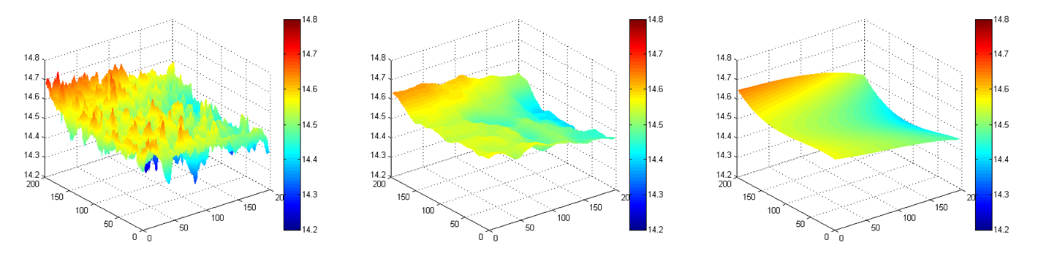
\includegraphics[width=16cm]{c4_plane_fit.png}
    \caption{基准面拟合效果图}
    \label{fig:c4_plane_fit}
    \end{figure*}

    \section{种子点提取}
    \esection{Seed Specification}
    基准面拟合结束后,对于图像中的每一个像素点都能够获得一个基准面深度值,然后我们利用基准面来生成种子点。若对于某个像素点,其基准面的深度值与原始深度值的差大于一个阈值,则被认为是一个种子点。种子点生成策略如下公式所示:
    \begin{eqnarray}
    S_d=\left\{i:d_{norm}\left(i\right)>f\left(i\right)+T_{depth}\right\}
    \end{eqnarray}
    其中$S_d$表示缺陷种子点集合,$i$表示一个像素点,$d_{norm}\left(i\right)$ 和$f\left(i\right)$分别表示该像素点的基准面的深度值和深度图像的深度值, $T_{depth}$ 是一个阈值,该阈值需要根据缺陷的深度定义来确定。
    \section{基于种子点的图像分割}
    \esection{Seed based Image Segmentation}
    获得种子点之后,下一步就是在深度图像上使用基于种子点的图像分割算法,可以采用的方法有很多,例如:Graph cut\cite{Boykov2001Interactive, Boykov2001Fast}、random walker\cite{Grady2006Random}、SFM 水平集\cite{Lankton2009Sparse}和Fuzzy connectedness\cite{Udupa2014Body, Udupa1996Disclaimer}等等。经过实验,我们选择SFM 水平集方法作为最后的分割算法,因为该方法的效果最好,能够有效的应对噪声。

    SFM水平集属于主动轮廓方法,主动轮廓图像分割方法能够迭代地演化一个轮廓从而尽可能一张图像分割成多个连通区域,达到图像分割的效果。SFM水平集的方法非常流行,主要是因为该类方法实现比较简单,并且能够拟合出足够复杂的模型。在SFM 水平集理论框架中,水平集轮廓可以理解为被包含在更高维度的函数中,比如一个二维平面中的轮廓$C$可以表示为三维空间中的函数$\phi$,按照惯例轮廓$C$可以表示成三维空间中函数$\phi$的零水平集,当$\phi<0$时,表示轮廓$C$的内部,当$\phi>0$时,代表轮廓$C$的外部区域。如图\ref{fig:c4_level_set}所示,这里给出一个例子,假设轮廓$C$ 是一个圆圈,那么对应的函数$\phi$的零水平集正好与轮廓$C$相匹配。

    \begin{figure*}[!h]
    \centering
    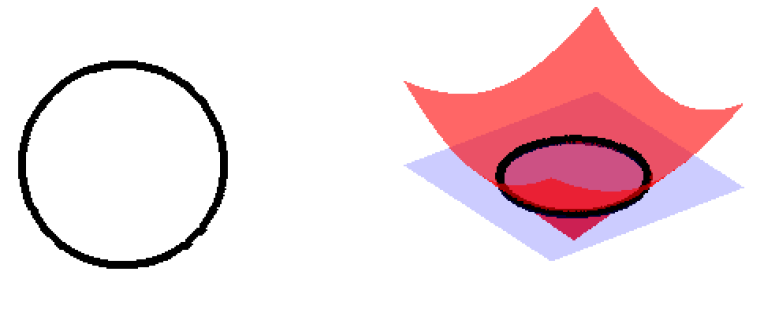
\includegraphics[width=16cm]{c4_level_set.png}
    \caption{SFM水平集理论示意图}
    \label{fig:c4_level_set}
    \end{figure*}

    SFM 水平集采用的是迭代的思路,基于局部信息不断扩大或者缩小水平集,相比较其他分割算法而言更为关注局部信息。SFM水平集算法通过不停的迭代修改0水平集的轮廓来最小化Chan-Vese能量函数\cite{Chan2001Active},Chan-Vese能量函数主要被用于主动轮廓模型领域,其函数形式如下:
    \begin{eqnarray}
    E=\int_{interior}\left({I-\mu_1}\right)^{2}+\int_{exterior}\left({I-\mu_2}\right)^{2}
    \end{eqnarray}
    SFM水平集分割算法结果如图\ref{fig:c4_SFM}所示,从左至右依次为深度图像三维伪彩图、提取的种子点图像、分割后的二值图像。

    \begin{figure*}[!h]
    \centering
    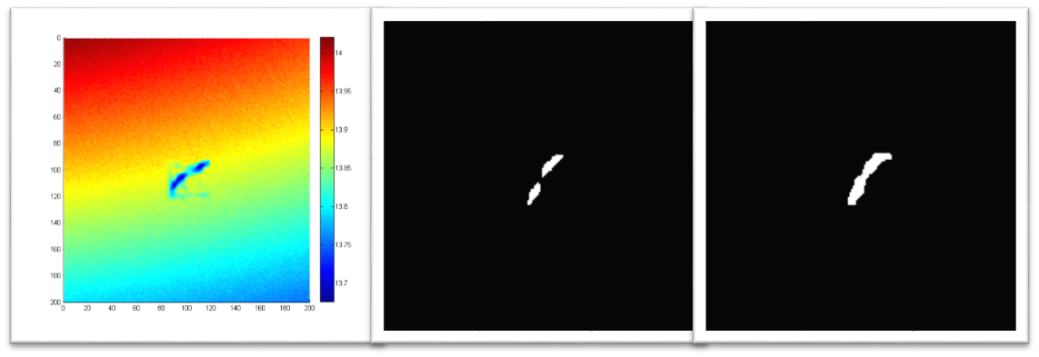
\includegraphics[width=12cm]{c4_SFM.png}
    \caption{SFM水平集分割算法效果图}
    \label{fig:c4_SFM}
    \end{figure*}

    \section{实验结果}
    \esection{Experimental Results}
        \subsection{数据集与评价方法}
        \esubsection{Data-set and Evaluation Protocol}
        目前采集到的钢板深度图像数据有限,为了能够对本文中提出的两种深度图像缺陷检测算法进行评价,利用真实的钢板深度图像我们采用人工合成的手段构建了一个钢板深度图像数据集。我们首先使用结构光3D扫描技术采集到一些带缺陷的钢板点云数据,然后将这些点云数据进行插值和裁剪处理转化为了深度图像。

        利用这些真实的带缺陷的钢板深度数据我们使用人工合成手段创建了一个深度图像数据集,该数据集一共有500张深度图像,图像的分辨率为1000x1000,缺陷数量总共有1489个。创建的流程主要为:

        1)根据真实钢板深度图像生成钢板模型;

        2)根据真实深度图像上的缺陷区域生成缺陷模型,另外也采用高斯函数生成了部分缺陷模型;

        3)随机选择钢板模型和缺陷模型,将钢板模型和缺陷模型组合起来生成合成深度图像。

        根据真实的钢板深度图像,首先随机提取100张1000x1000的子图,然后使用章节4.2中的基准面拟合方法拟合出这些子图的基准面,接着将这些基准面保存下来作为钢板模型。部分钢板模型的三维伪彩图如图\ref{fig:c4_steel_model}所示。

        \begin{figure*}[!h]
        \centering
        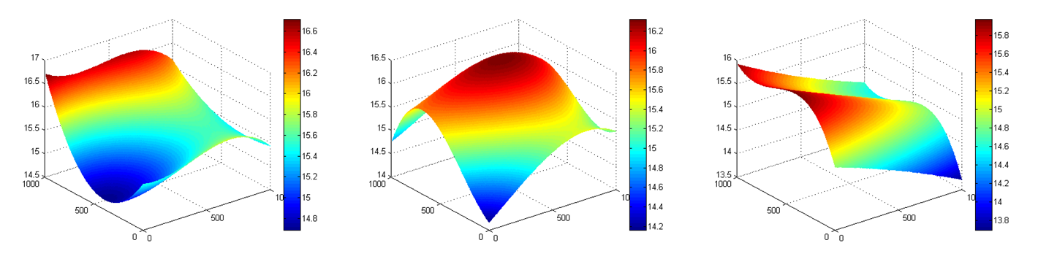
\includegraphics[width=16cm]{c4_steel_model.png}
        \caption{部分钢板模型三维伪彩图}
        \label{fig:c4_steel_model}
        \end{figure*}

        在真实的钢板深度图像上,我们使用人工标记的方法标记了缺陷区域,然后计算出这些缺陷区域与基准面的深度偏差,接着对深度偏差进行归一化,使得最大深度偏差等于缺陷的深度定义$D_{depth}$,然后归一化的深度偏差被保存作为缺陷模型。另外,我们也使用二维高斯函数生成了一些缺陷模型,最终一共生成了12 种缺陷模型。部分缺陷模型的三维伪彩图如图\ref{fig:c4_defect_model}所示:

        \begin{figure*}[!h]
        \centering
        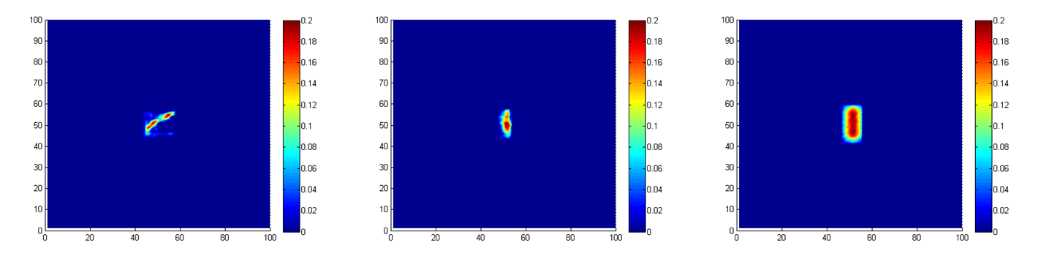
\includegraphics[width=16cm]{c4_defect_model.png}
        \caption{部分缺陷模型三维伪彩图}
        \label{fig:c4_defect_model}
        \end{figure*}

        最后,随机选择一个钢板模型和若干缺陷模型,对于每个缺陷模型,都采用参数随机的尺度变换和旋转变换来生成一个新的缺陷模型,尺度变换的尺度参数从0.5到2,步长为0.5,旋转变换的角度参数从0到360,步长为30。然后随机选择缺陷位置,将钢板模型减去缺陷模型获得带缺陷的钢板深度图像。

        对于检测算法检出的一个缺陷连通区域,我们使用连通区域包围盒的重叠率来判断检测是否成功,假定$R_p$为检测算法检测出的缺陷连通区域包围盒,$R_t$ 是已标记的缺陷连通区域包围盒,若$\frac{{R_p}\bigcap{R_t}}{{R_p}\bigcup{R_t}}>T_{overlap}$,即包围盒重叠率大于某个阈值则认为检测算法检出的该连通区域是一个缺陷。我们使用查全率、查准率和F 值来评价算法的最终检测效果。
        \subsection{实验结果与分析}
        \esubsection{Experimental Results and Analysis}
        我们使用Matlab语言实现了本文提出的两个深度图像缺陷检测算法,实验用的计算机配置为:Intel Xeon E3-1241 3.50GHz CPU、32GB内存、Windows 7操作系统。处理一张1000x1000的深度图像,基于基准面的方法平均处理时间为38s,使用了C++代码实现并增加多线程策略后,基于基准面的方法平均处理时间降低为500ms。

        移动曲面拟合方法首先对图像进行局部平滑处理,然后对每一个局部小窗口使用最小二乘法拟合局部曲面函数。使用MATLAB 语言实现的部分代码如下所示,这部分代码实现了基于移动曲面拟合方法来拟合基准面。

        \lstinputlisting{code/local_fitting_simple.m}

        Shepard方法基本思想是将待定点的函数值定义为拟合半径范围内各数据点函数值的加权平均,各数据点的权重按其距待定点的距离计算。下面这部分代码实现了利用Shepard方法来拟合基准面。

        \lstinputlisting{code/local_fitting_shepard.m}

        基于基准面的缺陷检测方法尝试去寻找钢板的基准面,然后将与基准面深度差别较大的区域作为缺陷种子点提取出来,最后使用基于种子点的图割方法来提取出完整的缺陷区域。下面这部分代码体现了基于基准面拟合方法检测缺陷的完整流程。

        \lstinputlisting{code/fitting_detect_defect.m}

        本章中提出的基于基准面拟合的深度图像缺陷检测算法在人工合成深度图像数据集上进行了实验,并评估了实验结果,实验结果如表\ref{tbl:c4_plane_result}所示:

        \begin{table*}[!h]
        \centering
        \caption{基于基准面拟合方法的实验结果}
        \label{tbl:c4_plane_result}
        \begin{tabularx}{\columnwidth}{>{\centering\arraybackslash}X >{\centering\arraybackslash}X >{\centering\arraybackslash}X >{\centering\arraybackslash}X}
        \toprule
        方法 & 查全率 & 查准率 & F值 \\
        \midrule
        基于基准面拟合 & 0.951 & 0.878 & 0.913 \\
        \bottomrule
        \end{tabularx}
        \end{table*}

        在实验中,我们设法寻找一组对数据集中所有深度图像都适用的参数,下面给出我们实验后的最优参数。在人工合成深度数据库的步骤中,根据工程的要求,缺陷的深度定义$D_{depth}$设置为0.2mm。

        基于基准面的缺陷检测算法是一种基于滑动窗的方法,窗口的大小设置为200x200,步长设置为100,这样每两个相邻的窗口都有一半的重叠,确保缺陷检出的查全率。提取种子点时,深度偏差阈值$T_{depth}$设置为0.1mm。由于滑动窗口有重叠,最终检测出来的缺陷可能有重复,需要使用非极大值抑制去掉多余的检测结果。

        本章提出的基于基准面拟合的深度图像缺陷检测算法在人工合成的数据集上达到了令人满意的效果。基于基准面的方法查全率较高,基本上缺陷区域都能够被检测出来,并且,基于基准面的缺陷检测算法能够将缺陷区域的轮廓完整提取出来,这是由于该方法在最后一步使用了基于种子点的图像分割方法,但是由于图像分割方法并不一定每次分割都完全准确,有时候会产生一个缺陷区域被分割成多个缺陷区域的情况,这种不完整分割的情况较多,并且在实验中发现,基于基准面拟合的方法还存在误检的问题,主要是因为基准面拟合不是完全准确导致了其会出现误检情况,基准面拟合的函数曲面跟真实钢板曲面大体上是一致的,但是在图像的边缘部分,拟合的曲面偏差较大,综上问题最终的查准率相对较低。

        在人工合成数据集上的部分实验结果如图\ref{fig:c4_plane_result}所示,从左至右依次为带缺陷的深度图像三维伪彩图、标记的缺陷区域、基于基准面算法的检测结果。

        \begin{figure*}[!h]
        \centering
        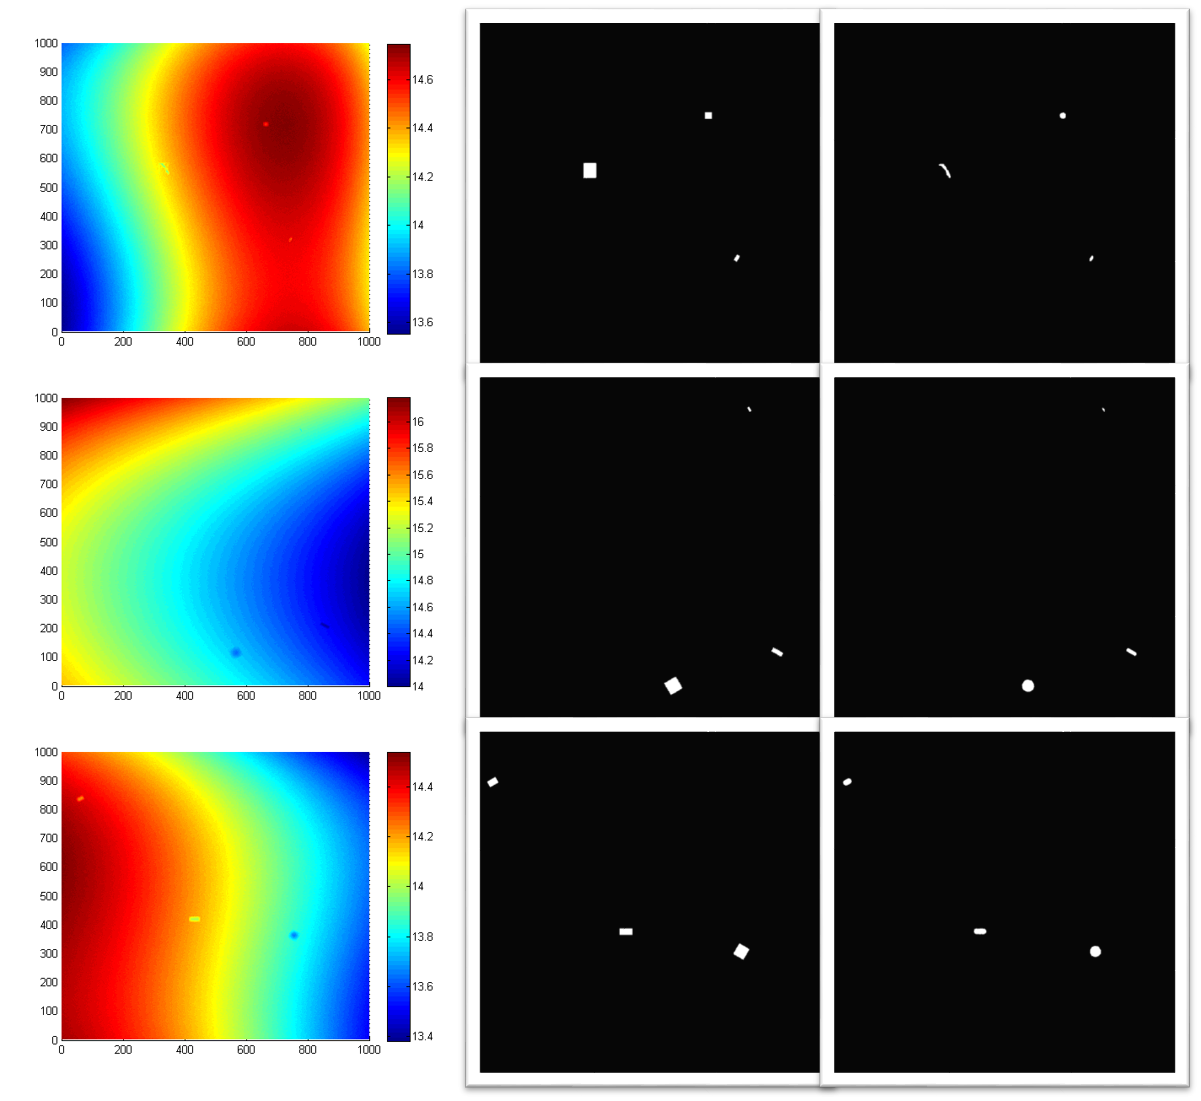
\includegraphics[width=16cm]{c4_plane_result.png}
        \caption{基于基准面拟合方法的部分实验结果}
        \label{fig:c4_plane_result}
        \end{figure*}

    \section{本章小结}
    \esection{Brief Summary}
    在本章中,我们提出了一种基于基准面拟合的深度图像缺陷检测算法。基于基准面的缺陷检测方法尝试去寻找钢板的基准面,然后将与基准面深度差别较大的区域作为缺陷种子点提取出来,最后使用基于种子点的图割方法来提取出完整的缺陷区域。

    另外,为了验证本文提出的两个缺陷检测算法,根据真实的钢板深度图像,我们使用人工合成的手段生成了一个钢板深度图像数据集,实验的结果显示,我们的方法达到了很好的效果。

